% -*- coding: utf-8; -*-

\chapter{Mapeamento}

\section{Linhas de Mapeamento}

Um dos recursos presentes no Sistema Recon é a \textbf{linha de mapeamento}, cujo objetivo é auxiliar na interpretação dos resultados gerados na restauração do modelo. Essa linha armazena referências a pontos topológicos da malha da seção. Com isso, é possível ter uma linha que acompanha a movimentação da malha de um cenário a outro.

As linhas de mapeamento (Figura~\ref{fig-linemap}) permitem realizar um mapeamento geométrico ao longo de uma restauração tomando como base uma linha-guia poligonal definida pelo usuário. Essa linha pode ser criada em qualquer cenário, mesmo em seções já restauradas.

\begin{figure} [h]
  \begin{center}
    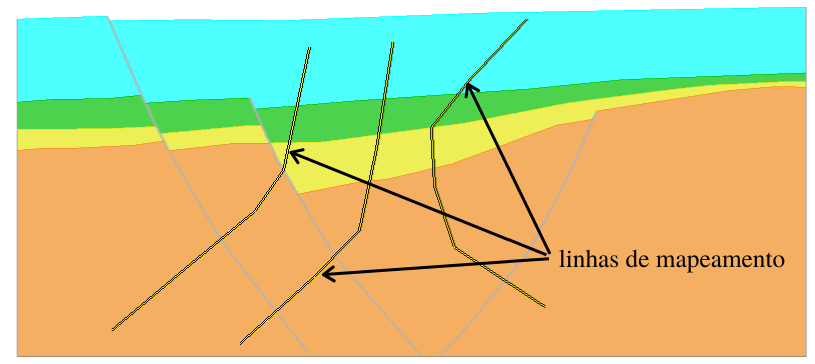
\includegraphics[width=400pt]{images/fig-linhas-de-mapeamento-ed}
    \caption{Linhas de mapeamento em uma seção.}\label{fig-linemap}
  \end{center}
\end{figure}

A Figura~\ref{fig-linemap-history} apresenta o resultado após uma transformação do tipo \textit{Move-Sobre-Falha} onde é possível observar, além da deformação da camada, a linha de mapeamento sofrendo a mesma movimentação. Este tipo de uso pode ser interpretado como se houvesse ali um falso horizonte para avaliar o quantidade de movimento na restauração do rejeito.

\begin{figure} [h]
  \begin{center}
    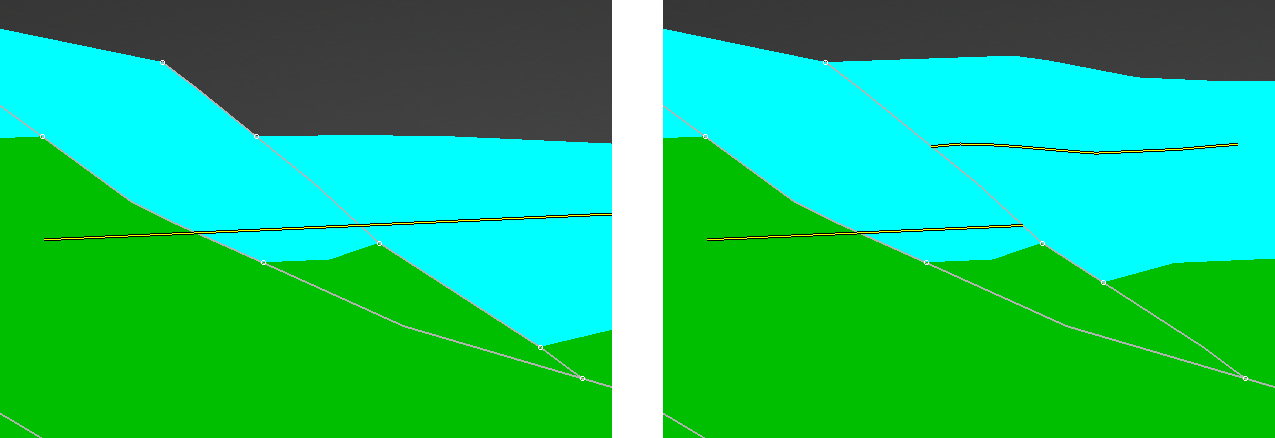
\includegraphics[width=420pt]{images/fig-linemap-history}
    \caption{Linhas de mapeamento em diferentes etapas}\label{fig-linemap-history}
  \end{center}
\end{figure}


Cada face de uma seção tem como atributo uma malha triangulada, e as linhas de mapeamento são definidas no sistema de coordenadas local da malha de cada uma das faces. Além disso, é possível que uma linha de mapeamento cruze diversas malhas, por isso, a linha de mapeamento é definida como um conjunto de \quotes{partes de linha de mapeamento} ou \textit{LineMapPart}, sendo cada parte pertencente a um trecho contínuo em uma mesma face. O processo de criação deste mapeamento da linha é feito para cada parte indidulmente, de forma que ao visualizar as partes tem-se a linha de mapeamento completa. Na Figura~\ref{fig-linemap-malhas} é possível ver uma linha de mapeamento cortando algumas malhas diferentes.

\begin{figure} [h]
  \begin{center}
    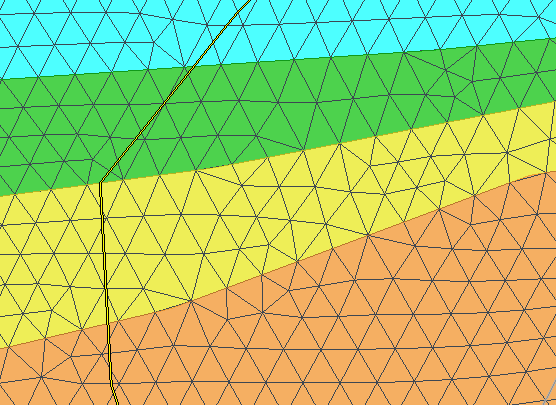
\includegraphics[width=250pt]{images/fig-linhas-de-mapeamento-malhas}
    \caption{Linhas de mapeamento cortando múltiplas faces.}\label{fig-linemap-malhas}
  \end{center}
\end{figure}

O primeiro passo na criação do mapeamento é a determinação da linha-guia pelo usuário, a partir disso é feita a separação nas partes a serem processadas de acordo com o número de faces interceptadas. É realizado um levantamento com informações topológicas da interseção da parte com a malha da face. Essa ação consiste em fazer uma relação entre um ponto da parte da linha-guia e um ponto em uma entidade topológica da malha, seja ela um nó, aresta de elemento ou elemento triangular.

Por exemplo, na Figura~\ref{fig-linemap-parts} estão evidenciadas as partes que formam a linha de mapeamento. Cada uma dessas partes é representada pela entidade chamada \textit{LineMapPart}, termo apresentado anteriormente.

\begin{figure} [h]
  \begin{center}
    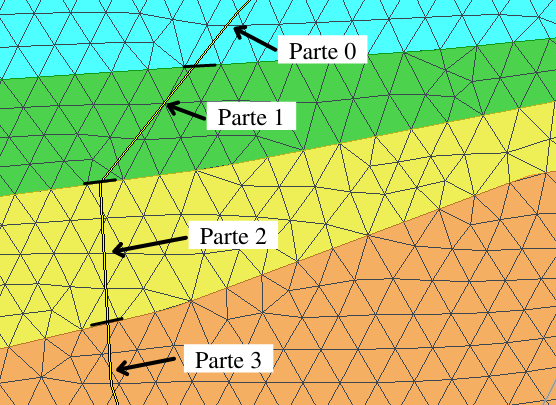
\includegraphics[width=250pt]{images/fig-lm-parts}
    \caption{Partes de uma linha de mapeamento}\label{fig-linemap-parts}
  \end{center}
\end{figure}

A malha das faces, por sua vez, possui três entidades básicas, o ponto da linha pode ser mapeado para um nó topológico, para um ponto interno de uma aresta (lado de triângulo) de uma malha ou ponto interior a um elemento (triângulo da malha). Em cada um desses casos, a informação topológica relacionada é guardada, segundo a enumeração a seguir:

\renewcommand{\labelitemi}{•}
\begin{itemize}
  \item Nó: guarda o indentificador do nó
  \item Aresta: guarda o identificador da aresta e a coordenada paramétrica do ponto de cruzamento.
  \item Elemento: guarda o identificador do elemento e as coordenadas baricêntricas do ponto no interior do elemento.
\end{itemize}

A Figura~\ref{fig-lm-topo} mostra a idenficação dos pontos em uma LineMapPart e a Tabela~\ref{tab-lm-topo} exibe quais informações topológicas são salvas de cada ponto.

\begin{figure} [hbt!]
  \begin{center}
    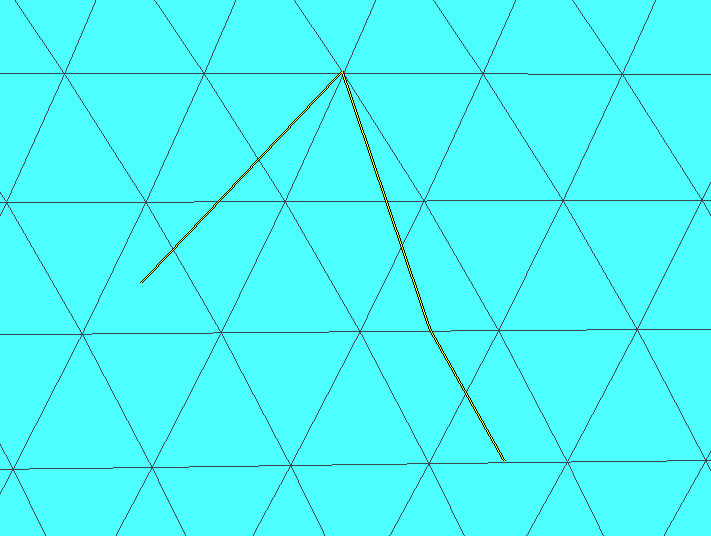
\includegraphics[width=260pt]{images/fig-lm-topo}
    \caption{Informações topológicas da malha mapeadas para a linha de mapeamento.}\label{fig-lm-topo}
  \end{center}
\end{figure}

% -*- coding: utf-8; -*-

\begin{table} [hbt!]
 \begin{center}
	 \caption{Informações topológicas salvas na linha de mapeamento.\label{tab-lm-topo}}
	~\\[-2mm]
	 \begin{tabularx}
		 {\textwidth}
		 {cp{2.0cm} lp{3.0cm} lp{10.0cm}}

		 \textbf{Ponto}
		 & \textbf{Tipo}
		 & \textbf{Informação armazenada} \\ \toprule

		 %~\\[-1mm]
		 A
		 & Elemento
		 & id=30, coordenadas baricêntricas=(0,33; 0,33; 0,33) \\ \midrule

		 %~\\[-1mm]
		 B
		 & Nó   
		 & id=431 \\ \midrule

		 %~\\[-1mm]
		 C
		 & Aresta
		 & id=130, coordenada paramétrica=0,45 \\ \midrule

		 %~\\[-1mm]
		 D
		 & Aresta
		 & id=145, coordenada paramétrica=0,55 \\ \midrule

	 \end{tabularx}
 \end{center}
\end{table}


Após esse processo de mapeamento topológico da linha propriamente dita, é possível calcular a geometria da linha em diferentes cenários que usam a mesma malha (já que a topologia é mantida), bastando apenas verificar se a malha se manteve, isto é, não foi refeita, apagada ou editada.

Em casos de edição, todos os atributos associados à malha são interpolados para a nova versão da malha, incluem-se nisso as partes de linha de mapeamento que recebem uma nova versão se a malha original teve sua topologia alterada.

A vantagem deste tipo de mapeamento é ser baseado em malha, já que todas as transformações geológicas que ocorrem no processo de restauração, do ponto de vista computacional, tem como objetivo deformar a malha.

\section{Derivações das Linhas de Mapeamento}

As linhas de mapeamento têm também casos de usos mais especializados, como na criação e representação de poços. Poços são criados semelhantemente às linhas de mapeamento ou por importação de modelos com poços em 3D. Possuem característica de serem linhas mais verticalizadas e possuem uma finalidade mais limitada. Nos casos de poços 3D, a linha correspondente ao poço é apenas uma projeção do objeto tridimensional no plano da seção.

Há o uso nas chamadas linhas de interseção (\textit{CrossLine}) que servem para identificar e mapear as linhas de cruzamento entre seções no espaço tridimensional do multi-seções, com isso é possível ter uma noção do que ocorre com seções transversais mesmo estando no domínio bidimensional da restauração.

\subsection{Linhas de Mapeamento do Modelo}

Por fim, as linhas de mapeamento são a base para a \textit{linhas de mapeamento do modelo} ou \textit{LMModel}, cujo objetivo é servir como um mapeamento das linhas de entidades geológicas (horizonte, falha e topo de sal) ao longo da restauração do modelo. Dessa forma, é possível ter um acompanhamento das entidades geológicas na seção, baseado no contorno da malha das faces que são mais bem discretizadas que as arestas originais da subdivisão planar, além de poder verificar como se deu a movimentação de cada ponto de horizonte ao longo da restauração, por exemplo.

Pelo objetivo proposto, as LMModels são linhas de mapeamento que tomam a geometria das entidades geológicas como entrada, então não há necessidade de criar uma linha-guia como é feita na linha de mapeamento original, a própria linha de horizonte ou falha é usada como linha-guia.

Além disso, há o armazenamento de atributos importantes para a manipulação das LMModels, como idade dos horizontes, identificador da falha e até sobre a qual pedaço de superfície aquela parte de linha está associada.

Todas essas informações  geológicas atreladas ao mapeamento topológico das LMModels, quando em conjunto com as diversas seções geológicas de um modelo multi-seções, são o que fazem dela o principal dado para a realização de um mapeamento de informações a nível 3D, já que trazem todo o histórico de movimentação das camadas de um modelo geológico.

A maneira de trabalhar com LMModels é com a organização dela em estruturas de dados que formam subconjuntos divididos por etapa de resturação e idade (caso de linhas de horizonte). Com isso é obtido o conjunto de informações que representam a restauração das seções de uma forma mais simples e fácil de se trabalhar a nível tridimensional.

\section{Mapeamento de superfícies}

\subsection{Metodologia}

\subsection{Preparação dos dados}

\subsection{Exemplos e resultados}

\section{Mapeamento do Volume}

\subsection{Metodologia}

\subsection{Preparação dos dados}

\subsection{Exemplos e resultados}


